%
% stabilitaet.tex -- Computational mode
%
% (c) 2020 Prof Dr Andreas Müller, Hochschule Rapperswio
%
\subsection{Stabilität und Computational Mode
\label{pde:subsection:stabilitaet}}
In der Diskussion des Wärmeleitungsproblems haben wir für die Zeitableitung
nicht versucht, symmetrische Differenzen zu verwenden.
Tatsächlich gibt es einen wichtigen Grund dafür, der in diesem Abschnitt
untersucht werden soll.
Es wird sich zeigen, dass symmetrische Differenzen zusätzliche instabile
Lösungen erzeugen können, die nichts mit realen Lösungen der
Differentialgleichung zu tun haben.
Dieser sogenannte {\em Computational Mode}
\index{Computational Mode}
führt auf nutzlose Resultate und dürfte mit ein Grund für die Misserfolge
von Lewis Fry Richardson in seinen Pionierversuchen zur numerischen
Wettervorhersage gewesen sein
\cite{buch:richardson}.

\subsubsection{Vorwärtsdifferenzen}
Zur Illustration des Problem verwenden wir die einfache Differentialgleichung
\[
y' = -y,\quad y(0)=y_0
\]
welche die wohlbekannte Lösung $y(x)=y_0e^{-x}$ hat.
Zur Diskretisation verwenden wir die Gitterpunkte $x_i=ih$, $i\in\mathbb Z$
und versuchen die Werte $y_i = y(x_i)$ zu berechnen.
Diskretisation mit Vorwärts-Differenzen führt auf 
\[
y'(x_i) \approx \frac{y_{i+1}-y_i}{h} = -y(x_i) = -y_i
\quad\Rightarrow\qquad
y_{i+1} = y_u-hy_i = (1-h)y_i.
\]
Damit kann man die Lösung als 
\[
y_i = y_0(1-h)^i
\]
schreiben.
Wählt man $h=x/n$, dann liefert diese Approximation
\[
y(x) = y_0\biggl(1-\frac{x}n\biggr)^n 
\to
y_0e^{-x}
\]
für $n\to\infty$.
Dieses Verfahren konvergiert also, wenn auch nicht besonders schnell,
da das Euler-Verfahren nur ein Verfahren erster Ordnung ist.

\subsubsection{Symmetrische Differenzen}
Eine Schwierigkeit der Verwendung von Vorwärts-Differenzen ist, dass
die Vorwärts-Differenz eher eine Approximation für $y'(x_i+h/2)$ ist,
nicht für $y'(x_i)$.
Wie früher gezeigt wurde, können symmetrische Differenzen die Ableitung
im Punkt $x_i$ besser darstellen.
Die zugehörige Differenzengleichung wird jetzt
\[
y'(x_i)
=
\frac{y_{i+1}-y_{i-1}}{2h}
=
-y(x_i)
=
-y_i
\qquad\Rightarrow\qquad
y_{i+1}+2hy_i-y_{i-1}=0.
\]
Ein Potenzansatz $x_i=\lambda^i$ liefert die charakteristische Gleichung
\[
\lambda^{i+1} +2h\lambda^i -\lambda^{i-1}
=
\lambda^{i-1}(\lambda^2 + 2h\lambda -1)
=
0
\]
mit den Lösungen
\[
\lambda_\pm = -h \pm \sqrt{h^2+1}.
\]
Die Quadratwurzel kann in die Taylor-Reihe
\[
\sqrt{1+h^2}
\approx
1 + \frac{h^2}2 + O(h^4)
\]
entwickelt werden.
Es folgt, dass $\lambda$-Wert für das positive Vorzeichen
\[
\lambda_+
=
-h+\sqrt{h^2+1}
\approx
1-h+\frac{h^2}{2}+\dots
<
1
\]
kleiner als $1$ ist, insbesondere ist die Folge $\lambda_+^i$ monoton fallend.

Verwenden wir wieder die Schrittweite $h=x/n$, dann ist
\[
y_i
=
y_0 \lambda_+^i
=
y_0 \biggl(1-h+\frac{h^2}2\biggr)^n
=
y_0\biggl(1-\frac{x}n + o(h)\biggr)^n
\to
y_0e^{-x}
\]
für $n\to\infty$, die Lösung für positives Vorzeichen liefert also genau
die gleiche Lösung, die wir bereits mit Vorwärtsdifferenzen gefunden haben.

Die zweite Lösung der charakteristischen Gleichung mit dem negativen
Vorzeichen ist
\[
\lambda_-
=
-\frac{h}2 - \sqrt{\frac{h^2}{4}+1}
<
-1.
\]
Die Lösungsfolge $\lambda_-^i$ hat alternierende Vorzeichen, aber die 
Beträge $|\lambda_-^i|$ wachsen exponentiell schnell an.
Die Verwendung symmetrischer Differenzen führt also dazu, dass die
Differenzengleichung eine zweite Lösung bekommt, die exponentiell
schnell anwächst.
Diese zweite Lösung heisst der {\em Computational Mode}.
\index{Computational Mode}

\subsubsection{Numerische Anregung des Computational Mode}
Man muss sich fragen, warum man sich über die zweite Lösung überhaupt
Gedanken machen soll, immerhin wird ja für die Lösung der
Differentialgleichung nur die Lösung $\lambda_+$ benötigt.
Der Grund ist, dass bei der Berechnung der Lösung mit Hilfe der
Rekursionsformel
\[
x_{i+1} = x_{i-1}-2hx_i
\]
die zweite Lösung trotzdem auftritt.
Zu zwei aufeinanderfolgenden Werten $y_0$ und $y_1$ kann man mit der
Rekursionsformel alle weiteren Werte berechnen.
Aber selbst wenn man $y_1 = \lambda+y_0$ setzt, wird die numerische
Rechnung Rundungsfehler einführen, so dass der Wert $y_1$, der für die
Rekursion verwendet wird, nicht mit dem exakten Wert $\lambda_+y_0$
übereinstimmt.
Wir nehmen an, dass dieser Rundungsfehler $\delta$ der einzige
Fehler ist, der im Laufe der Berechnung eingeführt wird.
Wir müssen also die exakte Lösung für die Startwerte $y_0$ und
$\lambda_+y_0+\delta$ bestimmen.
Es sind also Koeffizienten $a_\pm$ zu finden mit
\begin{align*}
a_+ + a_- &= y_0 \\
a_+\lambda_+ + a_-\lambda_-&=y_0\lambda_++\delta
\end{align*}
Subtrahiert man das $\lambda_+$-fache der ersten Gleichung von der
zweiten Gleichung, erhält man
\[
a_-(\lambda_-\lambda_+)=\delta
\qquad\Rightarrow\qquad
a_- = \frac{\delta}{\lambda_--\lambda_+} = -\frac{\delta}{h}.
\]
Es folgt, dass selbst ein einziger minimaler Fehler $\delta$
bei der Berechnung von $y_1$ die Lösung die zweite Lösung sichtbar
macht. 

Man kann auch ausrechnen, wie gross $i$ werden muss, bis der
Computational Mode von der gleichen Grössenordnung wie die
gesuchte Lösung geworden ist.
Dieser Fall tritt ein wenn
\[
|y_0\lambda_+^i| < |\delta\lambda_-^i|
\qquad\Rightarrow\qquad
\biggl|
\frac{\lambda_-}{\lambda_+}
\biggr|^i
> \biggl|\frac{y_0}{\delta}\biggr|
\quad\Rightarrow\quad
i
>
\frac{\log |y_0/\delta|}{\log|\lambda_-/\lambda_+|}.
\]
Für kleine Werte von $h$ ist
\[
\log |\lambda_\pm|
=
\log(1\mp h+o(h)) 
\approx
\mp h.
\]
Die Bedingung an $i$ kann man damit mit
\[
i \gtrsim \frac{\log |y_0/\delta|}{2h}
\]
approximieren.
Der $x$-Wert, bei dem der Computational Mode überhand nimmt, ist daher
\[
x \gtrsim h \frac{\log|y_0/\delta|}{2h} = \frac12(\log|y_0|-\log|\delta|)
\]
Für den \texttt{double}-Typ ist $|\delta| \approx 10^{-15}$,
das Verfahren ist also grundsätzlich nicht in der Lage, vernünftige
Resultate für $x>7.5\log 10\approx 17.269$ zu liefern.

\begin{figure}
\centering
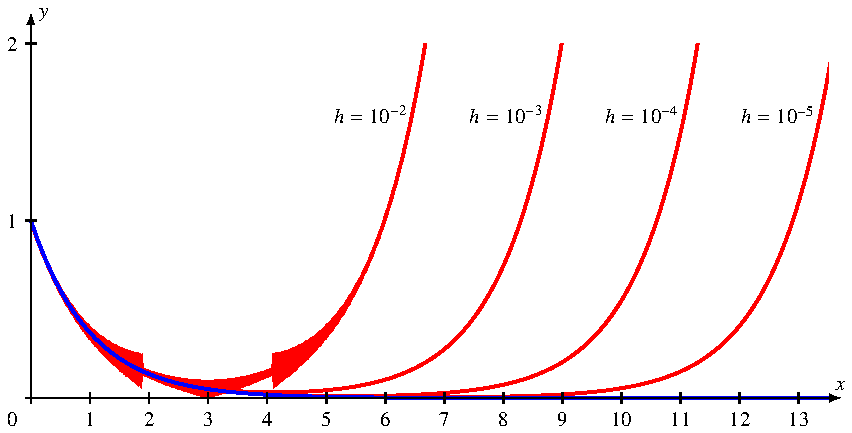
\includegraphics{chapters/70-pde/experiments/computationalmode.pdf}
\caption{Betrag der Lösung der Differentialgleichung $y'=-y$ berechnet
mit Hilfe symmetrischer Differenzen.
\label{buch:pde:cm:fig}}
\end{figure}
Die Annahme, der einzige Fehler trete bei der Rundung von $y_1$ auf,
ist natürlich viel zu optimistisch.
In Wahrheit tritt in jedem Schritt ein Fehler auf, so dass der 
Computational Mode schon viel früher angeregt wird.
In Abbildung~\ref{buch:pde:cm:fig} ist der Betrag der Lösung
für verschiedene Schrittweiten $h$ gezeigt.
Ganz zu Beginn, für $x<1$, scheint die Lösung einigermassen genau dem
theoretisch zu erwartenden Verlauf zu entsprechen.
Dann beginnt jedoch der Computational Mode überhand zu nehmen,
die Lösung wächst exponentiell schnell an und wird unbrauchbar.

Mehr Information zum Computational Mode insbesondere auch zu einer
Filtertechnik, mit der der Computational Mode auch wieder gedämpft
werden kann, ist im Kapitel~\ref{chapter:burgers} zu finden.







